\subsubsection{Compensación con Filtro de Kalman}

Dado que el filtro de Kalman puede estimar con precisión un estado en base a sucesivas mediciones, podemos utilizarlo para ubicar en todo momento al robot en el plano con su coordenada y velocidad estimadas. Esta información la podemos utilizar para determinar la corrección necesaria a aplicar para que el robot corrija su trayectoria, procederemos a describir este proceso.

Vale aclarar que el robot recibe comandos del siguiente formato, donde se especifica la distancia a recorrer con un vector determinado:
$$ [distancia, v_x, v_y, v_\theta] $$

Por otra parte el robot reporta el feedback de modo que es apto para el filtro de Kalman:
$$ [x, v_x, y, v_y] $$

\paragraph{Compensación espacial y vectorial} \mbox{} \vspace{10pt}

La compensación espacial y vectorial del robot omnidireccional se logra aprovechando las capacidades del filtro de Kalman para estimar el estado actual del sistema en tiempo real. Con esta información, el sistema puede ajustar los vectores de movimiento en las ruedas, compensando automáticamente irregularidades en el desplazamiento.

La corrección de la \textit{posición} del robot se realiza principalmente a través del filtro de Kalman, que combina el modelo cinemático con las mediciones reales para determinar en todo momento la ubicación exacta del robot en el espacio y su velocidad. Cuando se detectan desviaciones en la posición estimada, el filtro ajusta la estimación para reducir el error acumulado y garantizar un control óptimo.

Por otro lado, la \textit{trayectoria} planeada se corrige utilizando el modelo cinemático del robot. Este modelo define las relaciones entre los vectores de movimiento de las ruedas y los desplazamientos deseados en el espacio. Cuando el filtro de Kalman detecta desviaciones en la posición real, el sistema utiliza esta información para recalcular y corregir la trayectoria, asegurando que el robot siga el camino previamente definido.

\paragraph{Implementación} \mbox{} \vspace{10pt}

\textbf{Compensación espacial} \mbox{} \vspace{10pt}

Para la compensación espacial necesitamos determinar $d_c$, que es la distancia a recorrer para corregir la posición y llegar a $B$.

Definimos la compensación para un desplazamiento en el eye $y$ del mapa, luego se comprueba que el proceso es el mismo para un desplazamiento en $x$. En primer lugar se definen tres puntos claves:

$$ A = (x_1, y_1) : \text{Punto de partida} $$
$$ B = (x_2, y_2) : \text{Punto de llegada} $$
$$ X_a = (x_a, y_a) : \text{Coordenada actual del robot estimada por Kalman} $$
$$ d_c = (d_{xc}, d_{yc}) : \text{Distancia de compensación} $$

\begin{figure}[H]
    \centering
    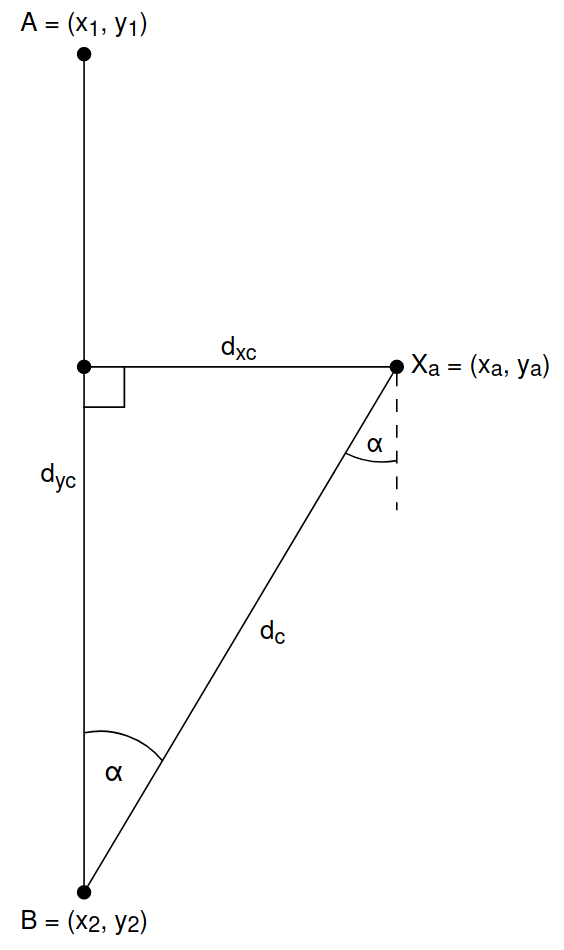
\includegraphics[width=0.4\linewidth]{images/compensacion_vector_distancia_kalman.png}
    \caption{Diagrama de compensación espacial}
    \label{fig:diagcompespacial}
\end{figure}

Para ello podemos definir:

$$ d_c = \sqrt{ {d_{xc}}^2 + {d_{yc}}^2 } $$
$$ d_{xc} = x_2 - x_a $$
$$ d_{yc} = y_2 - y_a $$

Con lo que podemos calcular $d_c$ para completar la tupla enviada al robot.

Ahora bien, en este punto podemos obtener el valor de $\alpha$:

$$ tan(\alpha) = \frac{d_{xc}}{d_{yc}} $$
$$ \alpha = arctan(\frac{d_{xc}}{d_{yc}}) $$

Es posible comprobar que para un desplazamiento sobre el eje $x$, la diferencia es que se calcula $\alpha$ de la siguiente manera:

$$ \alpha = arctan(\frac{d_{yc}}{d_{xc}}) $$

\textbf{Compensación vectorial} \mbox{} \vspace{10pt}

Para la compensación vectorial, en primera instancia definimos:

$$ V_c = (V_{xc}, V_{yc}) : \text{Vector de compensación} $$

\begin{figure}[H]
    \centering
    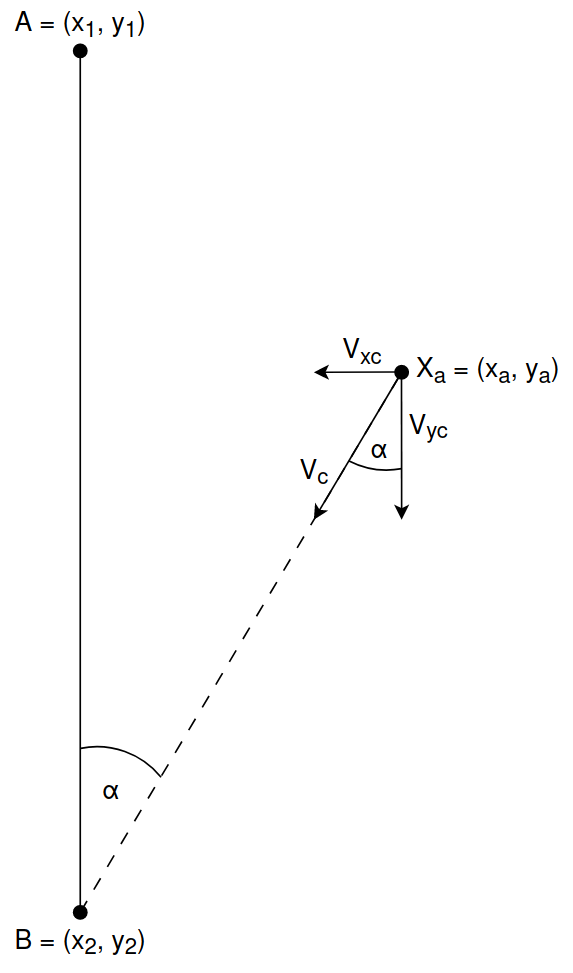
\includegraphics[width=0.4\linewidth]{images/compensacion_vector_velocidad_kalman.png}
    \caption{Diagrama de compensación vectorial}
    \label{fig:diagcompvectorial}
\end{figure}

Ahora bien, se establece que el valor de velocidad de compensación $V_c$ es constante, pero aún así necesitamos descomponer el vector para obtener $V_{xc}$ y $V_{yc}$ para enviarlo al robot:

$$ V_{xc} = V_c \cdot sen(\alpha) $$
$$ V_{yc} = V_c \cdot cos(\alpha) $$

Por lo que podemos definir:

$$ tan(\alpha) = \frac{V_{xc}}{V_{yc}} $$
$$ \alpha = arctan(\frac{V_{xc}}{V_{yc}}) $$

Con lo que ya podemos calcular $V_{xc}$ y $V_{yc}$ para enviarlo en la tupla que recibe el robot. En las tuplas del vector de compensación $v_\theta = 0$ dado que nuestro modelo de Kalman no contempla desplazamiento rotacional.

Es posible comprobar que para un desplazamiento sobre el eje $x$, la diferencia es que calculamos $\alpha$ de la siguiente manera:

$$ \alpha = arctan(\frac{V_{yc}}{V_{xc}}) $$